% Chapter 4: Methodology
\chapter{Methodology}

This chapter presents the comprehensive methodology used in the development of the Timetable Buddy system. It includes various modeling diagrams, project management artifacts, and quality assurance documentation that guided the system development process.

\section{Data Flow Diagrams (DFD)}

Data Flow Diagrams represent the flow of data through the system at different levels of abstraction, showing how information moves between processes, data stores, and external entities.

\subsection{DFD Level 0 (Context Diagram)}

The Context Diagram provides a high-level view of the entire Timetable Buddy system, showing its interaction with external entities including Students, Faculty, and Administrators.

\begin{figure}[h]
    \centering
    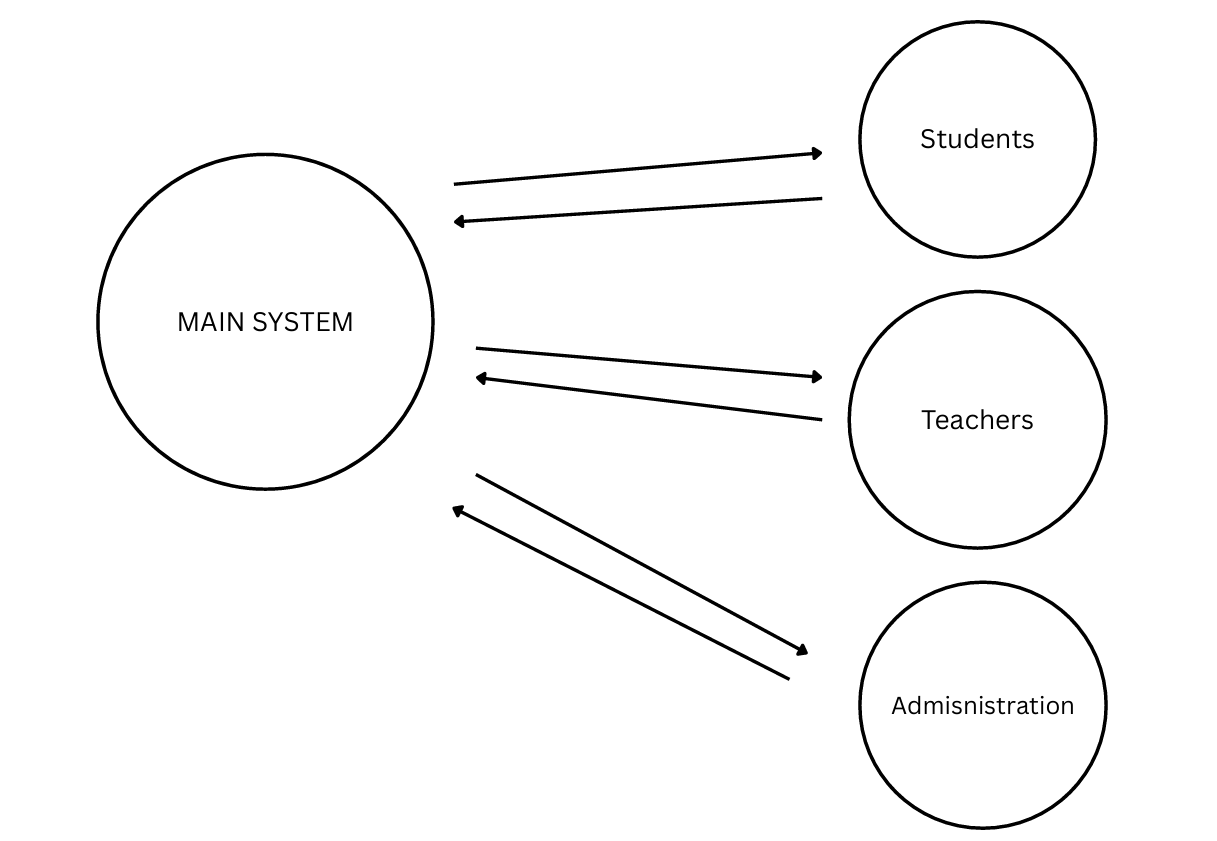
\includegraphics[width=0.85\textwidth]{images/DFD Level 0.png}
    \caption{DFD Level 0 - Context Diagram showing system boundaries and external entities}
    \label{fig:dfd0}
\end{figure}

The context diagram illustrates:
\begin{itemize}[leftmargin=*]
    \item \textbf{External Entities:} Students, Faculty, Administrators
    \item \textbf{Main System:} Timetable Buddy System (central process)
    \item \textbf{Data Flows:} Authentication requests, enrollment data, lecture schedules, timetable information
\end{itemize}

\subsection{DFD Level 1 (High-Level Processes)}

Level 1 DFD decomposes the main system into major processes, showing the primary functional components and their interactions.

\begin{figure}[h]
    \centering
    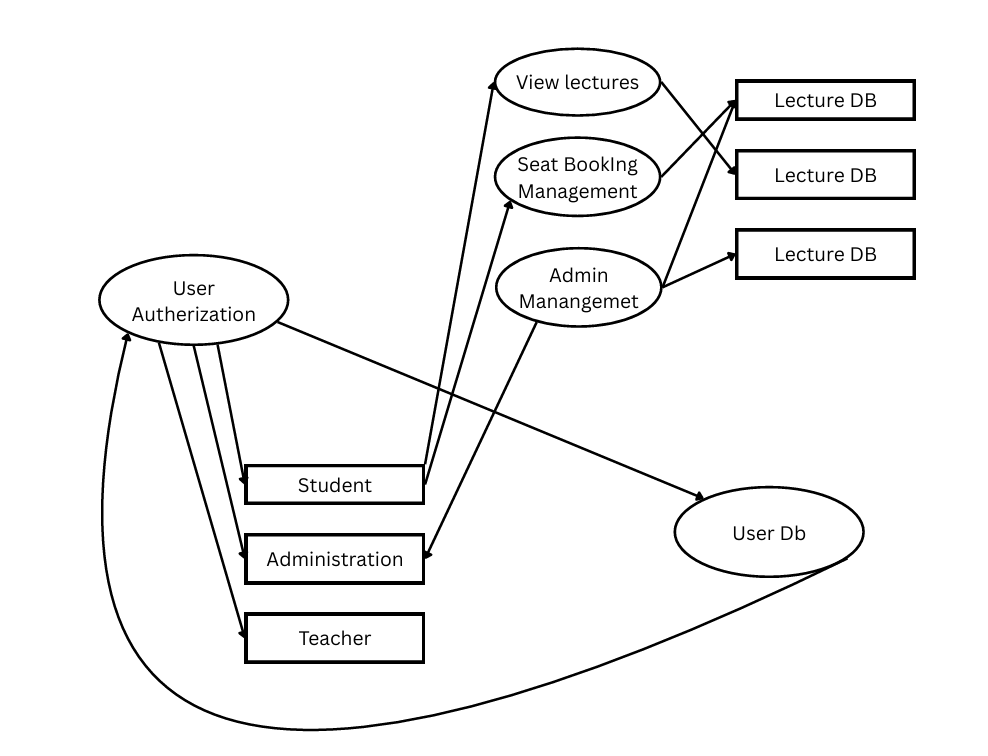
\includegraphics[width=0.95\textwidth]{images/DFD Level 1.png}
    \caption{DFD Level 1 - Major system processes and data stores}
    \label{fig:dfd1}
\end{figure}

Key processes shown in Level 1 include:
\begin{itemize}[leftmargin=*]
    \item User Authentication and Authorization
    \item Lecture Slot Management
    \item Enrollment Processing
    \item Timetable Generation
    \item Dashboard and Analytics
\end{itemize}

\subsection{DFD Level 2 (Detailed Processes)}

Level 2 DFD provides detailed decomposition of complex processes from Level 1, showing sub-processes and their interactions.

\begin{figure}[h]
    \centering
    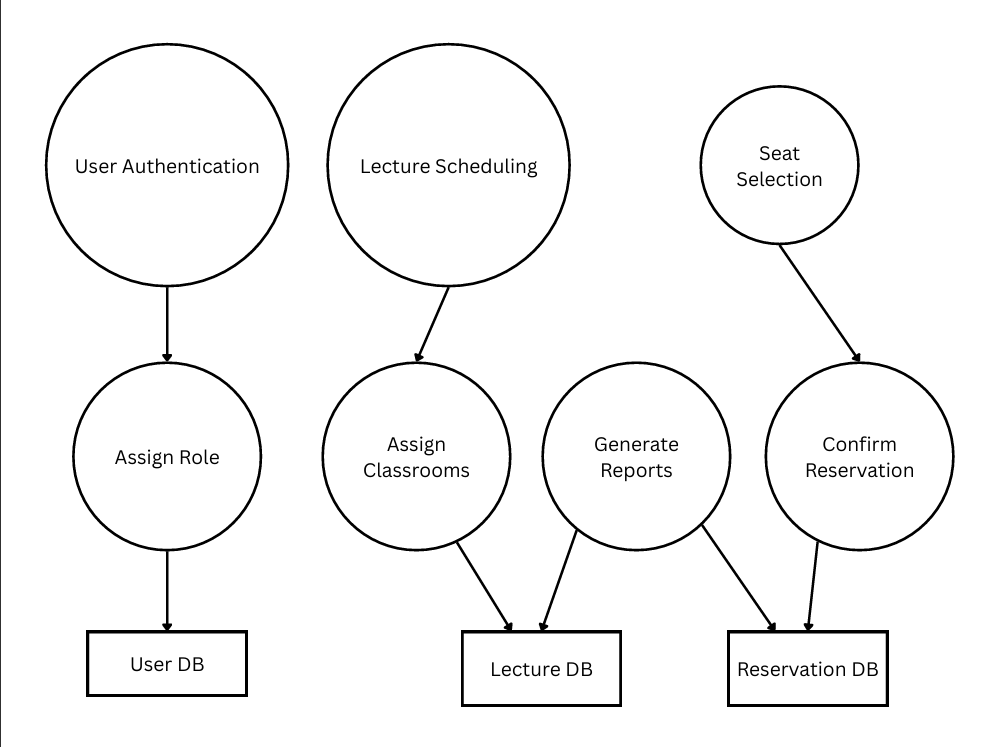
\includegraphics[width=0.95\textwidth]{images/DFD Level 2.png}
    \caption{DFD Level 2 - Detailed process decomposition}
    \label{fig:dfd2}
\end{figure}

The Level 2 diagram details:
\begin{itemize}[leftmargin=*]
    \item Enrollment workflow with waitlist management
    \item Conflict detection mechanisms
    \item Capacity validation processes
    \item Notification generation
\end{itemize}

\section{Use Case Diagram}

The Use Case Diagram illustrates the functional requirements from the user's perspective, showing the interactions between different actors and the system use cases.

\begin{figure}[h]
    \centering
    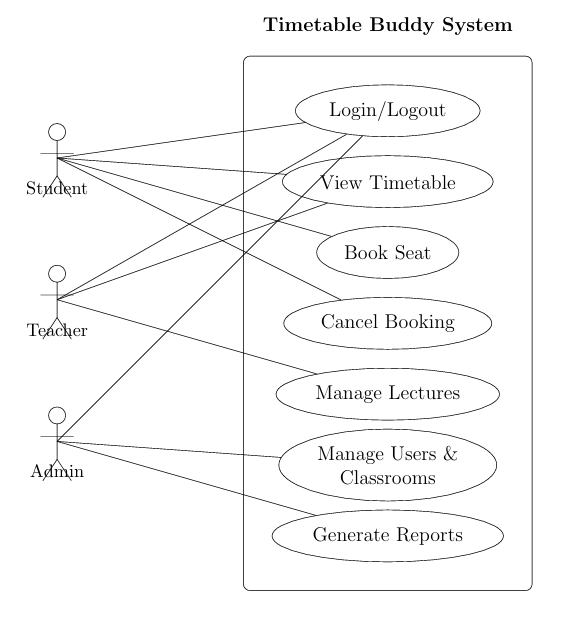
\includegraphics[width=0.85\textwidth]{images/Usecase diagram.png}
    \caption{Use Case Diagram showing actor interactions and system use cases}
    \label{fig:usecase}
\end{figure}

\textbf{Actors:}
\begin{itemize}[leftmargin=*]
    \item \textbf{Student:} Can view timetables, enroll in courses, manage profile, view enrollment status
    \item \textbf{Faculty:} Can manage lecture slots, view enrolled students, update course details
    \item \textbf{Administrator:} Can manage users, courses, lecture slots, generate reports, configure system settings
\end{itemize}

\textbf{Key Use Cases:}
\begin{itemize}[leftmargin=*]
    \item User Authentication (Login/Logout)
    \item Manage Lecture Slots
    \item Enroll in Courses
    \item View Timetable
    \item Manage Enrollments
    \item Generate Reports
    \item User Management
\end{itemize}

\section{Sequence Diagram}

Sequence Diagrams show the interaction between objects over time, illustrating the message flow and order of operations for specific scenarios.

\begin{figure}[h]
    \centering
    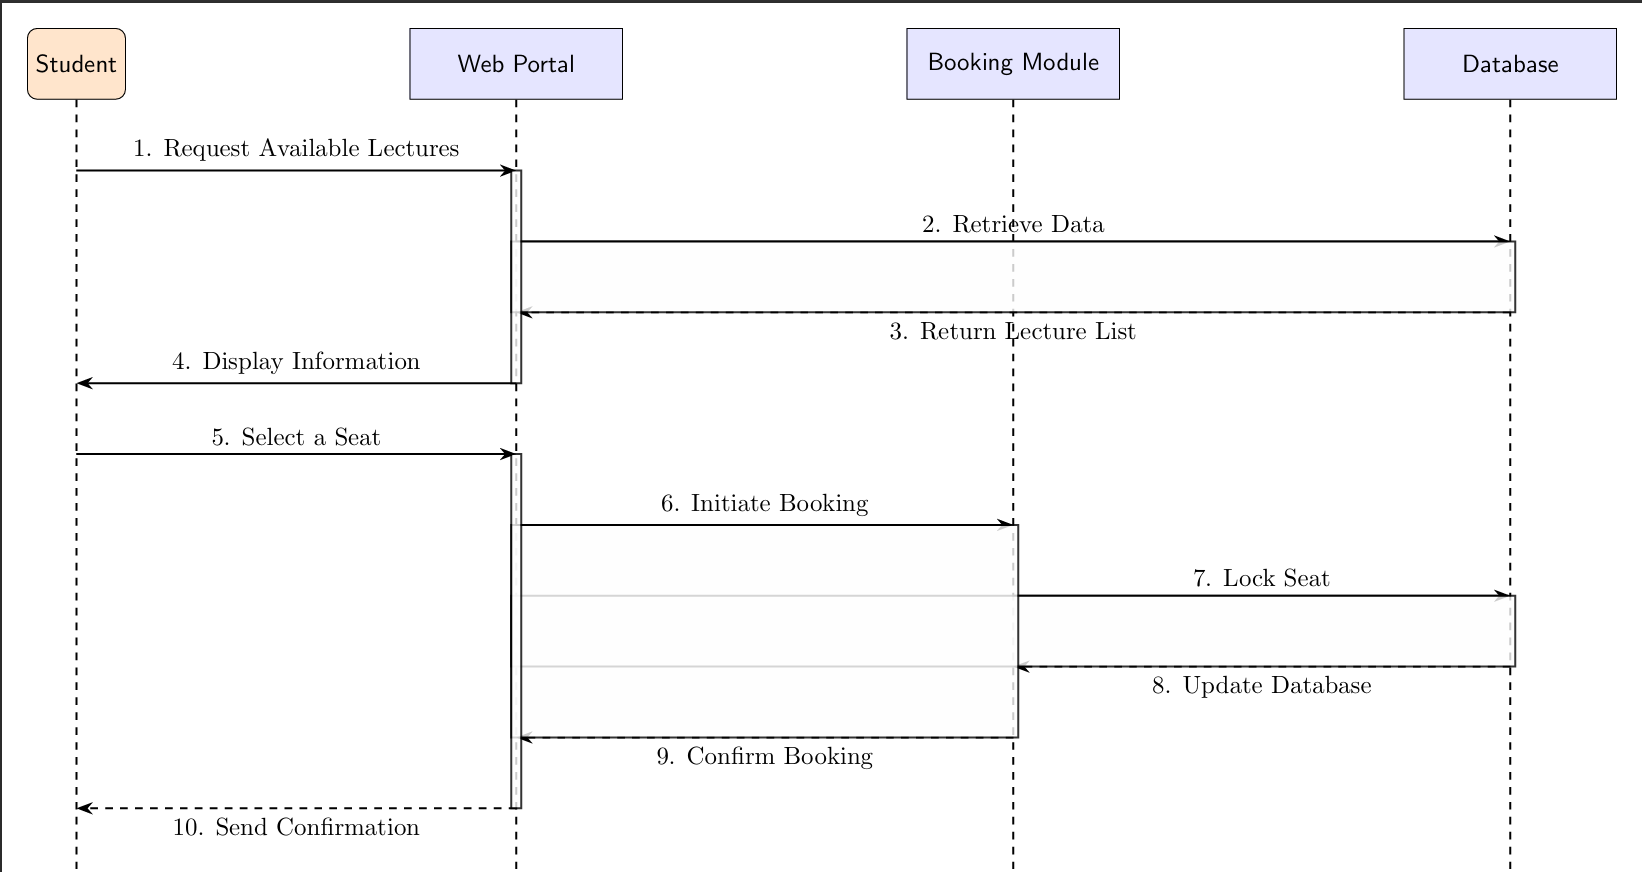
\includegraphics[width=0.95\textwidth]{images/Sequence Diagram.png}
    \caption{Sequence Diagram showing object interactions for enrollment process}
    \label{fig:sequence}
\end{figure}

The sequence diagram depicts:
\begin{itemize}[leftmargin=*]
    \item User authentication flow
    \item Enrollment request processing
    \item Conflict detection validation
    \item Capacity checking
    \item Database operations
    \item Response generation
\end{itemize}

\section{Activity Diagram}

Activity Diagrams model the workflow and business logic, showing the sequence of activities and decision points in system processes.

\begin{figure}[h]
    \centering
    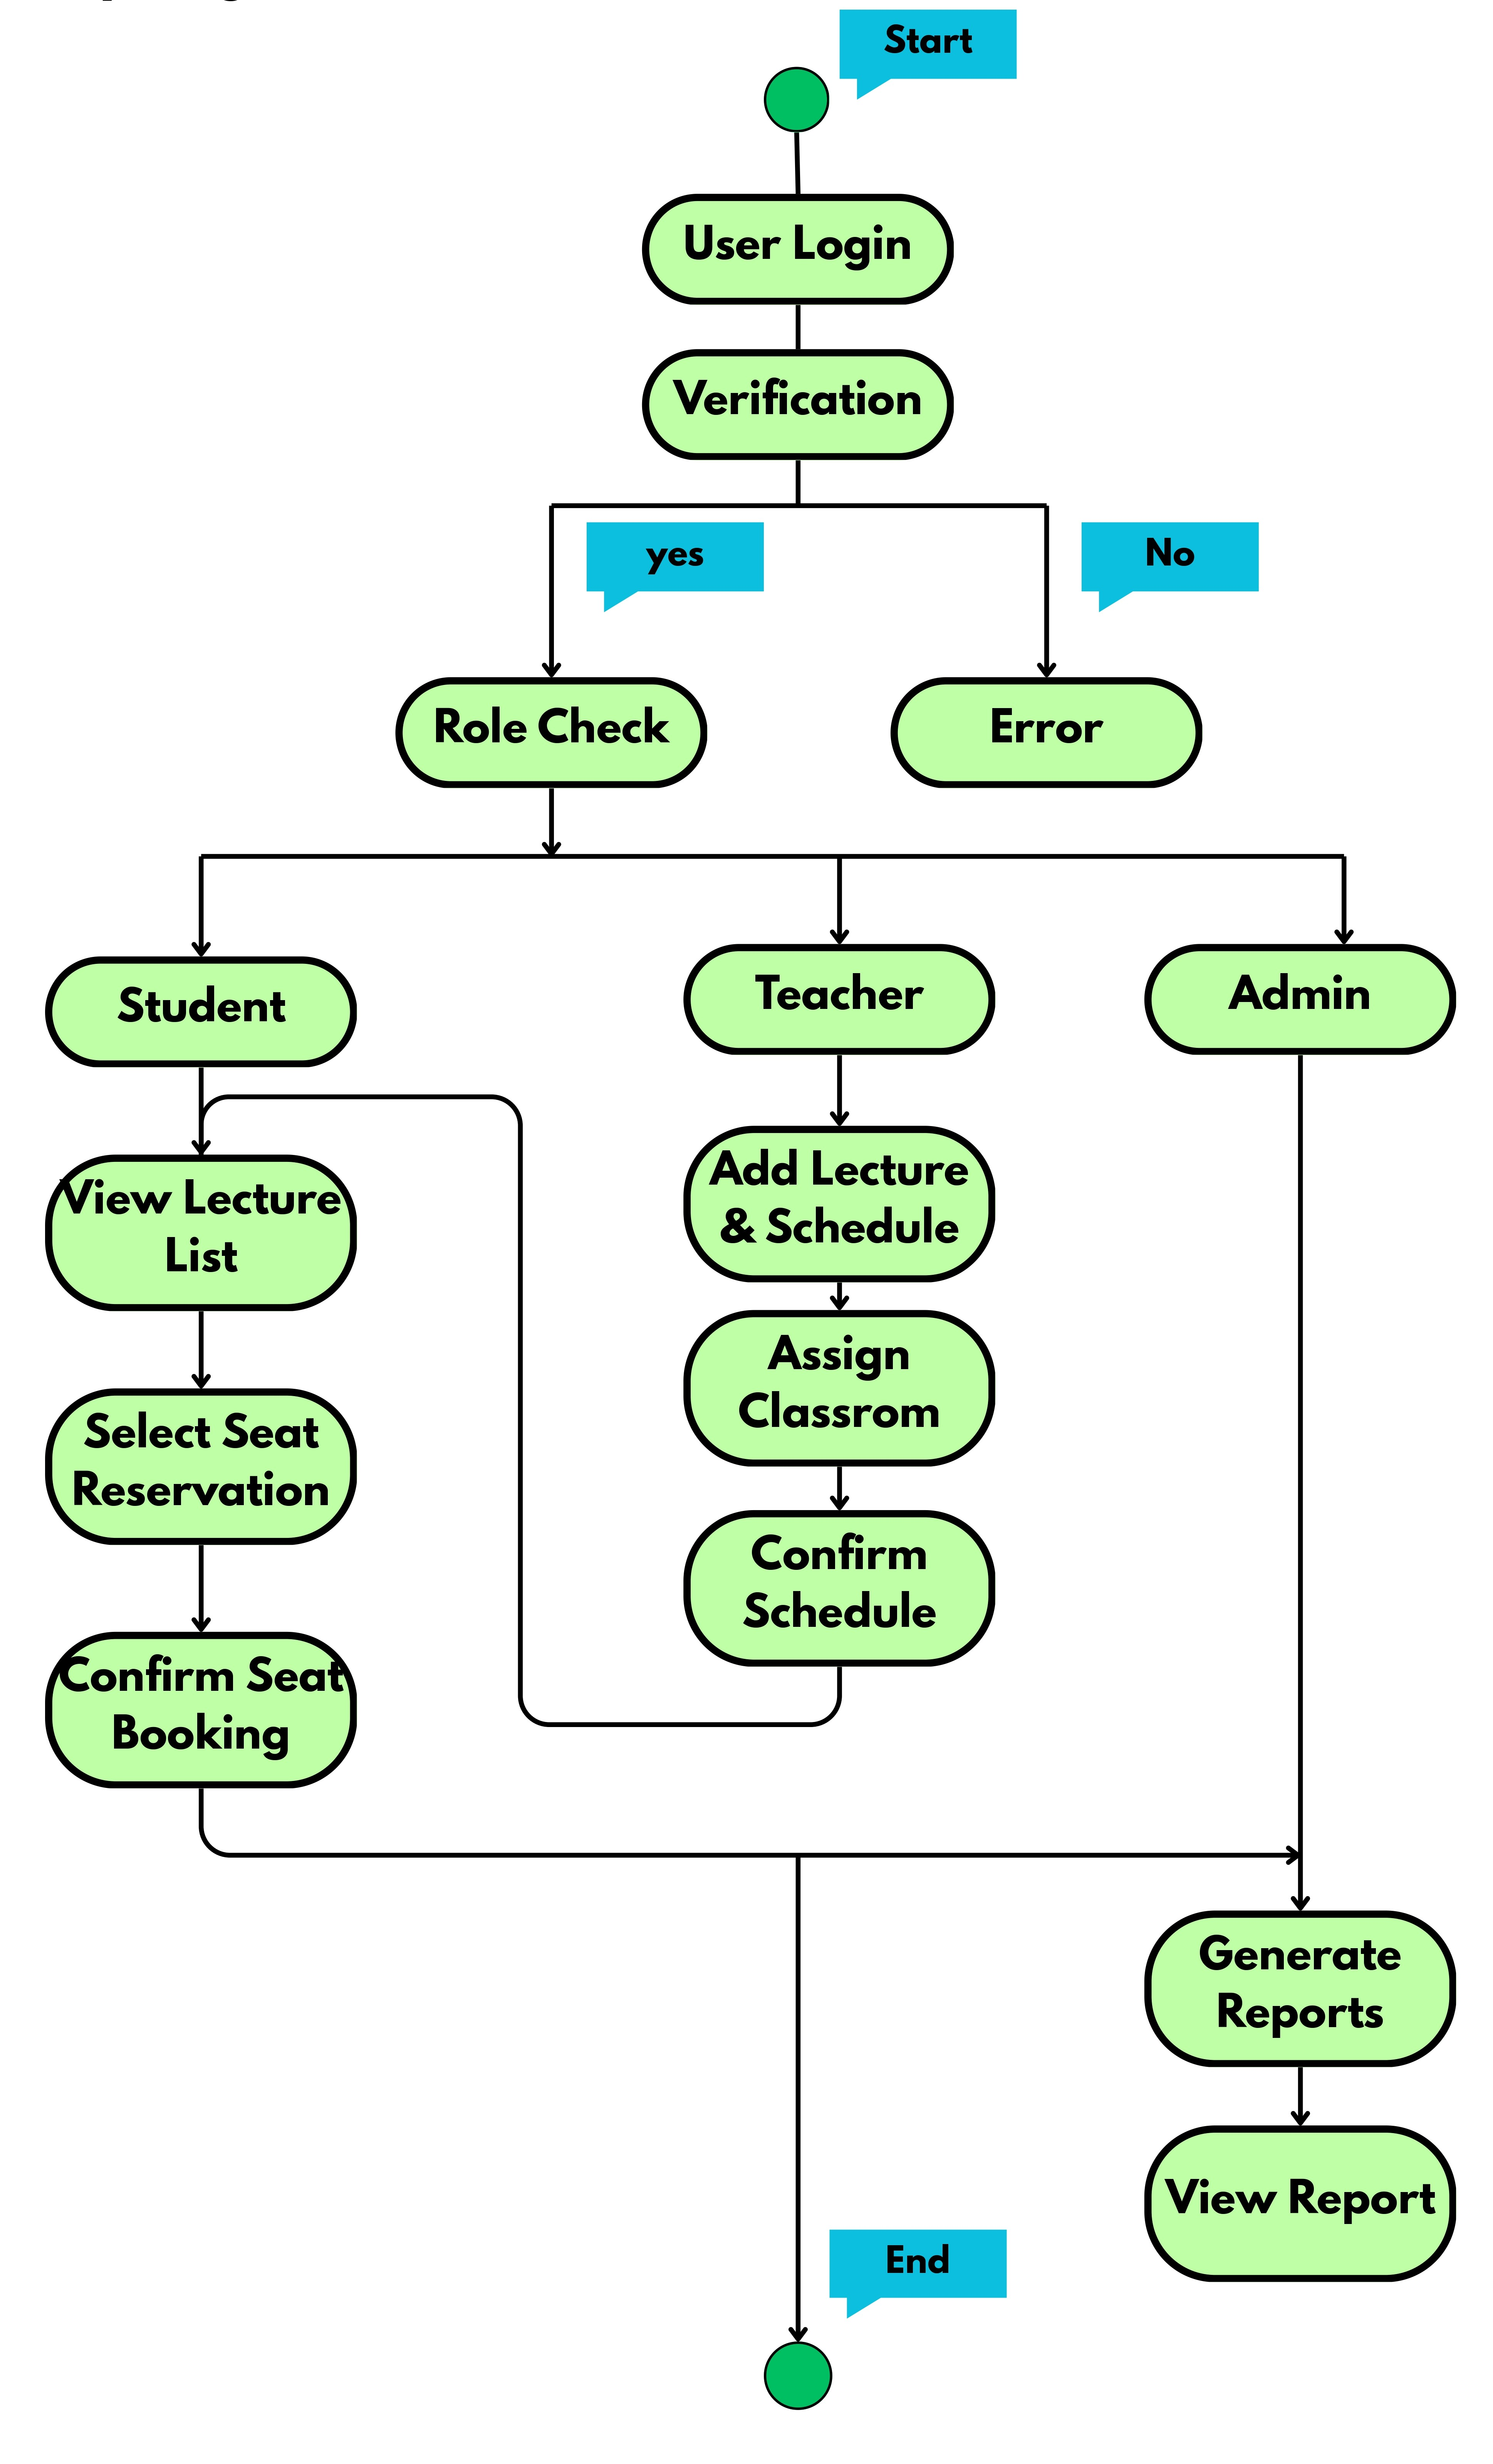
\includegraphics[width=0.75\textwidth]{images/Activity Diagram.jpg}
    \caption{Activity Diagram illustrating enrollment workflow and decision logic}
    \label{fig:activity}
\end{figure}

The activity diagram illustrates:
\begin{itemize}[leftmargin=*]
    \item Enrollment process workflow
    \item Decision points for capacity checks
    \item Conflict detection logic
    \item Waitlist management
    \item Success and failure paths
\end{itemize}

\section{Deployment Diagram}

The Deployment Diagram shows the physical architecture of the system, illustrating how software components are deployed on hardware nodes.

\begin{figure}[h]
    \centering
    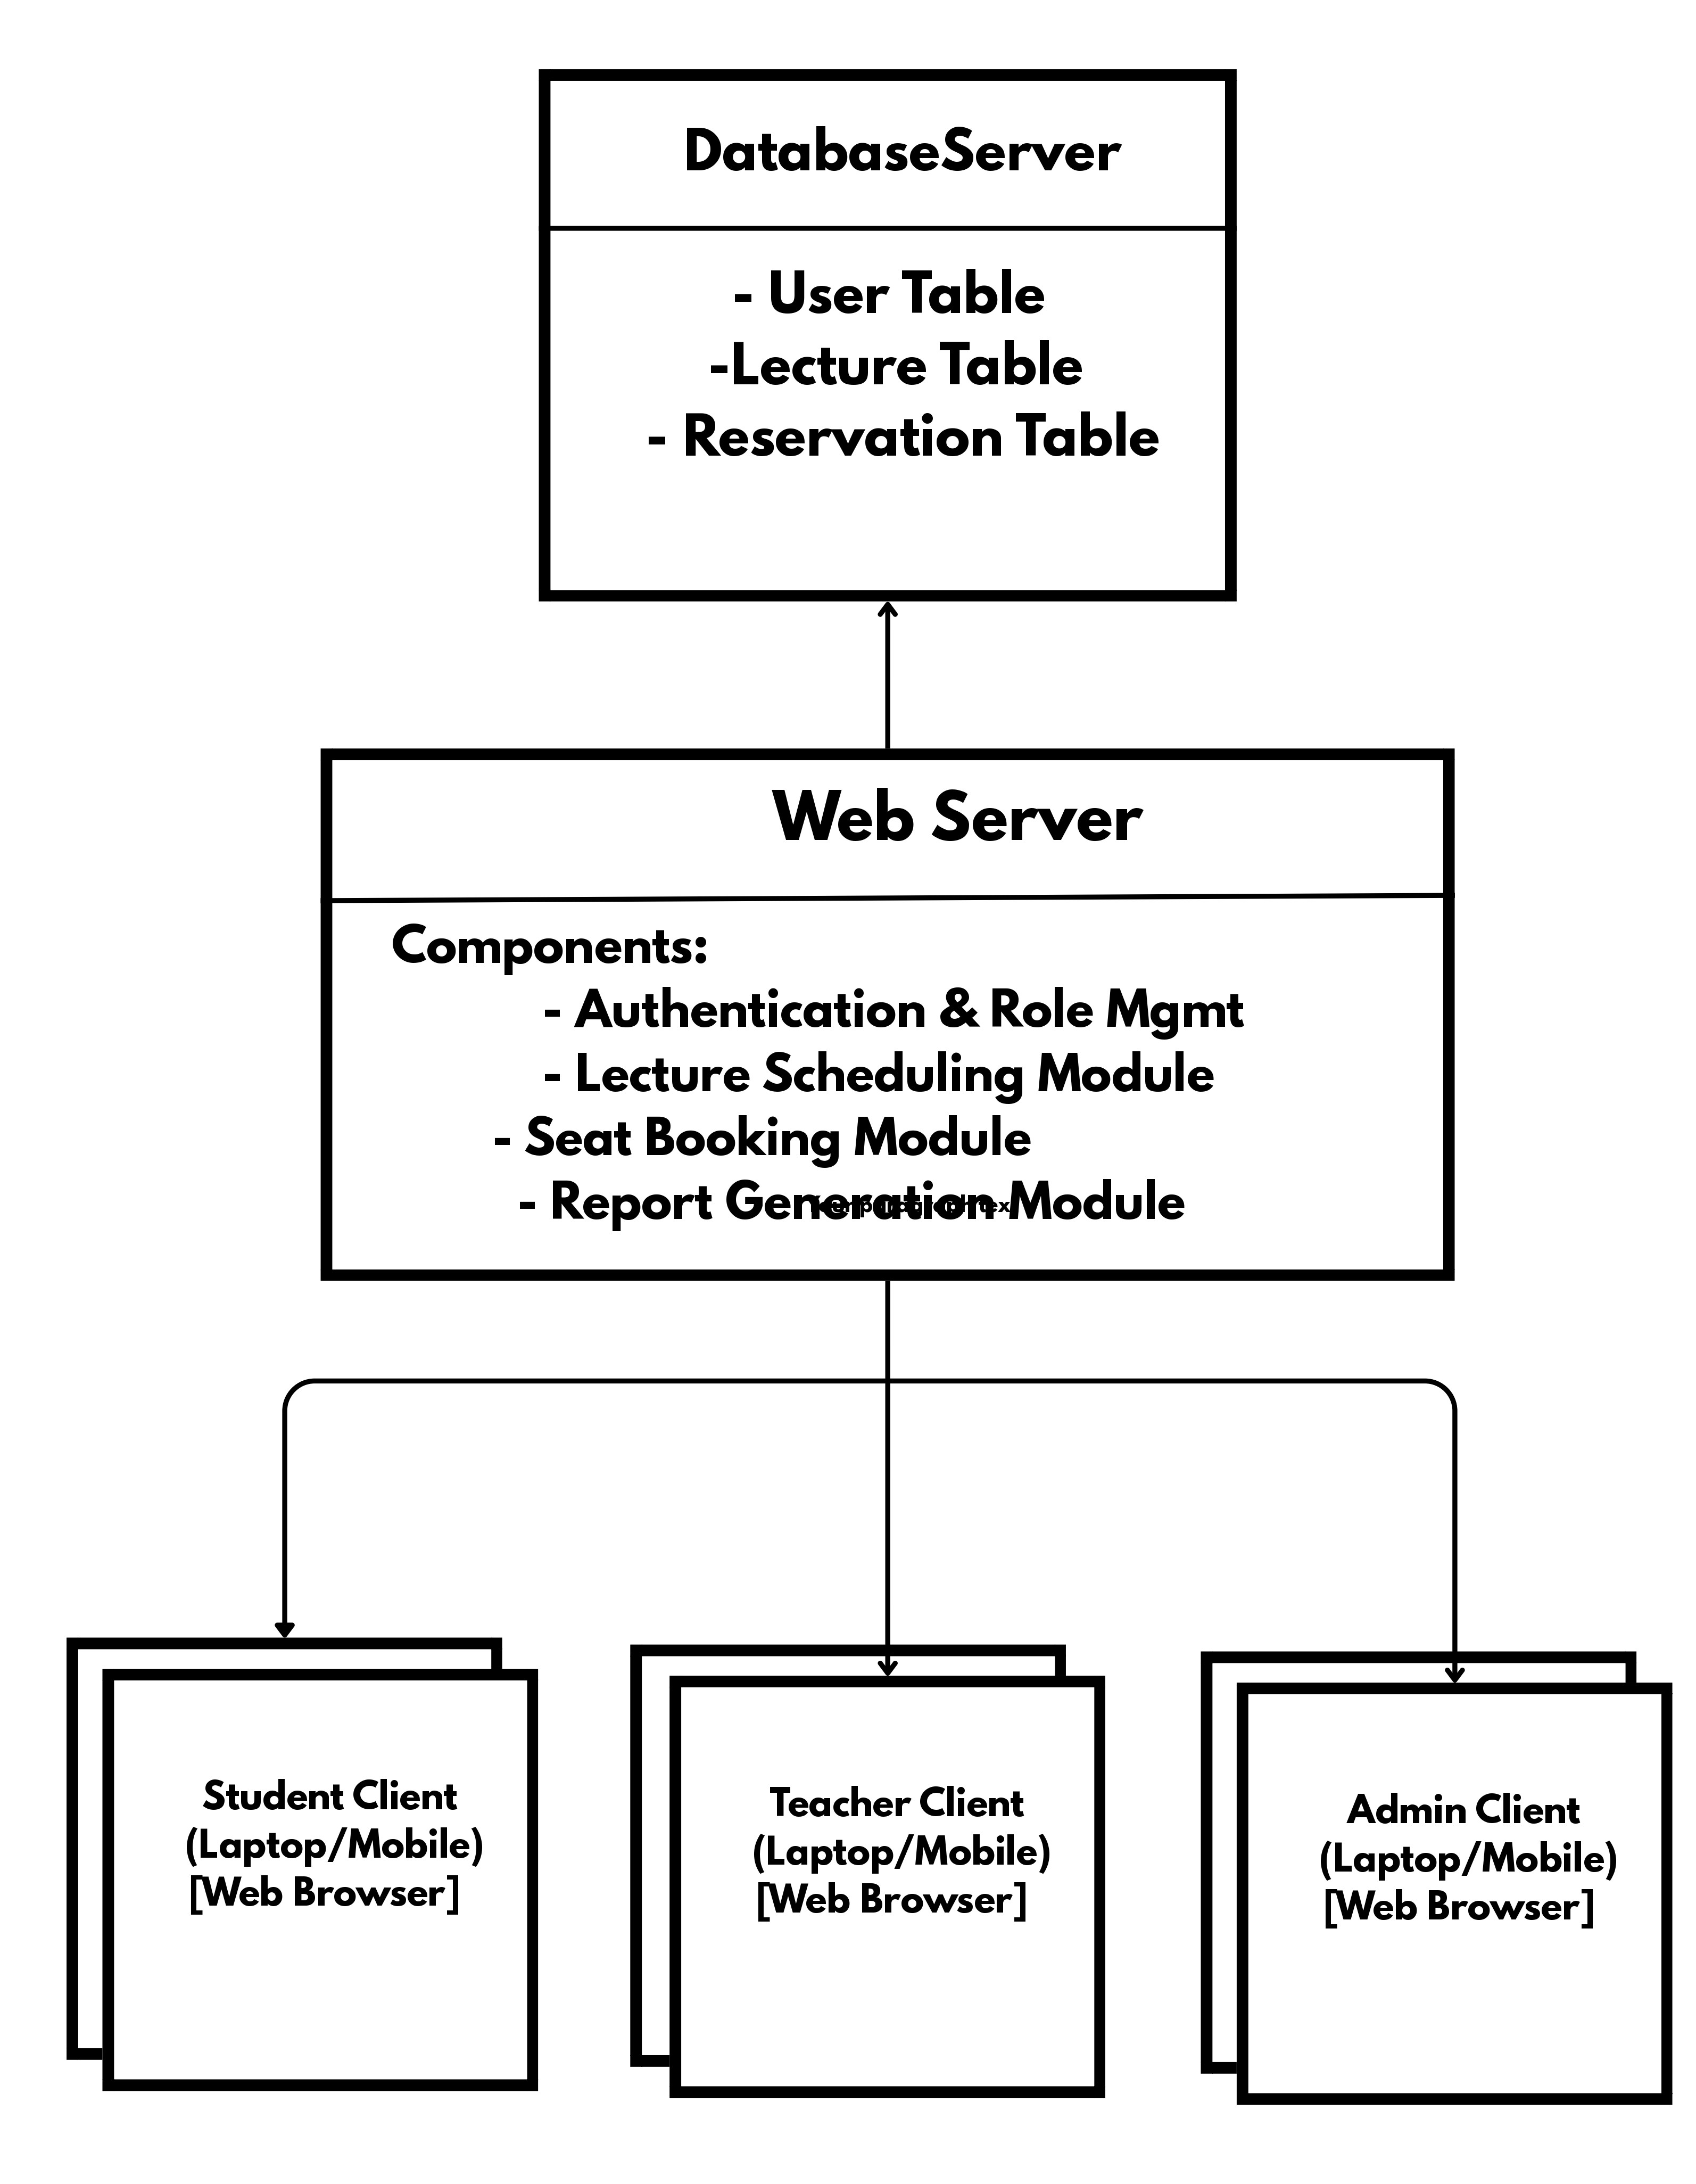
\includegraphics[width=0.85\textwidth]{images/Deployment Diagram.jpg}
    \caption{Deployment Diagram showing system architecture and component deployment}
    \label{fig:deployment}
\end{figure}

\textbf{System Components:}
\begin{itemize}[leftmargin=*]
    \item \textbf{Client Layer:} Web browsers on user devices
    \item \textbf{Application Layer:} React frontend, Node.js backend
    \item \textbf{Database Layer:} MongoDB database server
    \item \textbf{Deployment:} Docker containers for containerized deployment
\end{itemize}

\textbf{Communication Protocols:}
\begin{itemize}[leftmargin=*]
    \item HTTPS for client-server communication
    \item REST API for frontend-backend interaction
    \item MongoDB protocol for database connections
\end{itemize}

\section{Work Breakdown Structure (WBS)}

The Work Breakdown Structure decomposes the project into manageable components, showing the hierarchical breakdown of deliverables and tasks.

\begin{figure}[h]
    \centering
    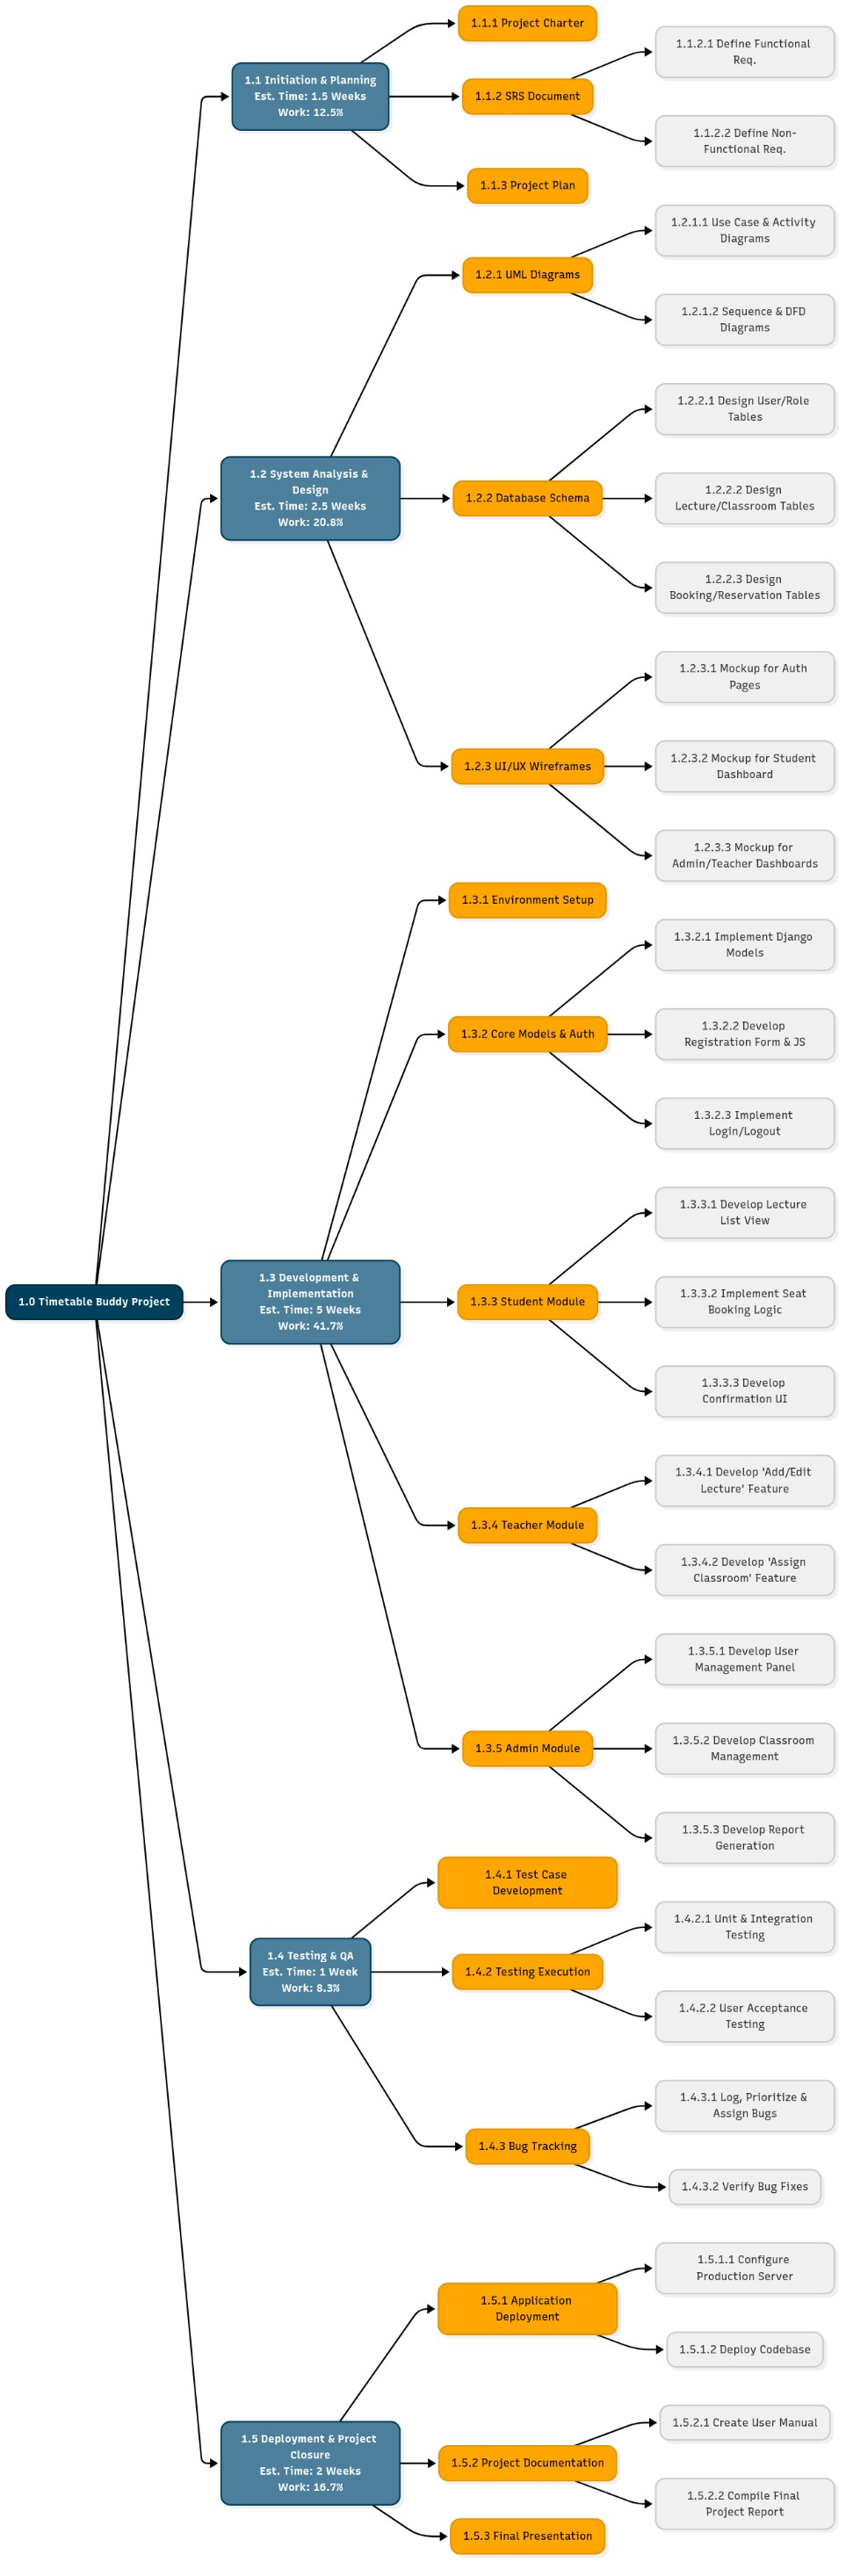
\includegraphics[width=0.95\textwidth]{images/WBS.jpg}
    \caption{Work Breakdown Structure showing project task hierarchy}
    \label{fig:wbs}
\end{figure}

\textbf{Major Work Packages:}
\begin{enumerate}[leftmargin=*]
    \item \textbf{Project Planning:} Requirements gathering, feasibility analysis, project plan
    \item \textbf{Design:} System architecture, database design, UI/UX design, API design
    \item \textbf{Development:} Frontend development, backend development, database implementation
    \item \textbf{Testing:} Unit testing, integration testing, system testing, user acceptance testing
    \item \textbf{Deployment:} Environment setup, deployment, documentation
    \item \textbf{Project Management:} Risk management, quality assurance, documentation
\end{enumerate}

\section{Gantt Chart}

The Gantt Chart provides a timeline view of project activities, showing task dependencies, durations, and milestones.

\begin{figure}[h]
    \centering
    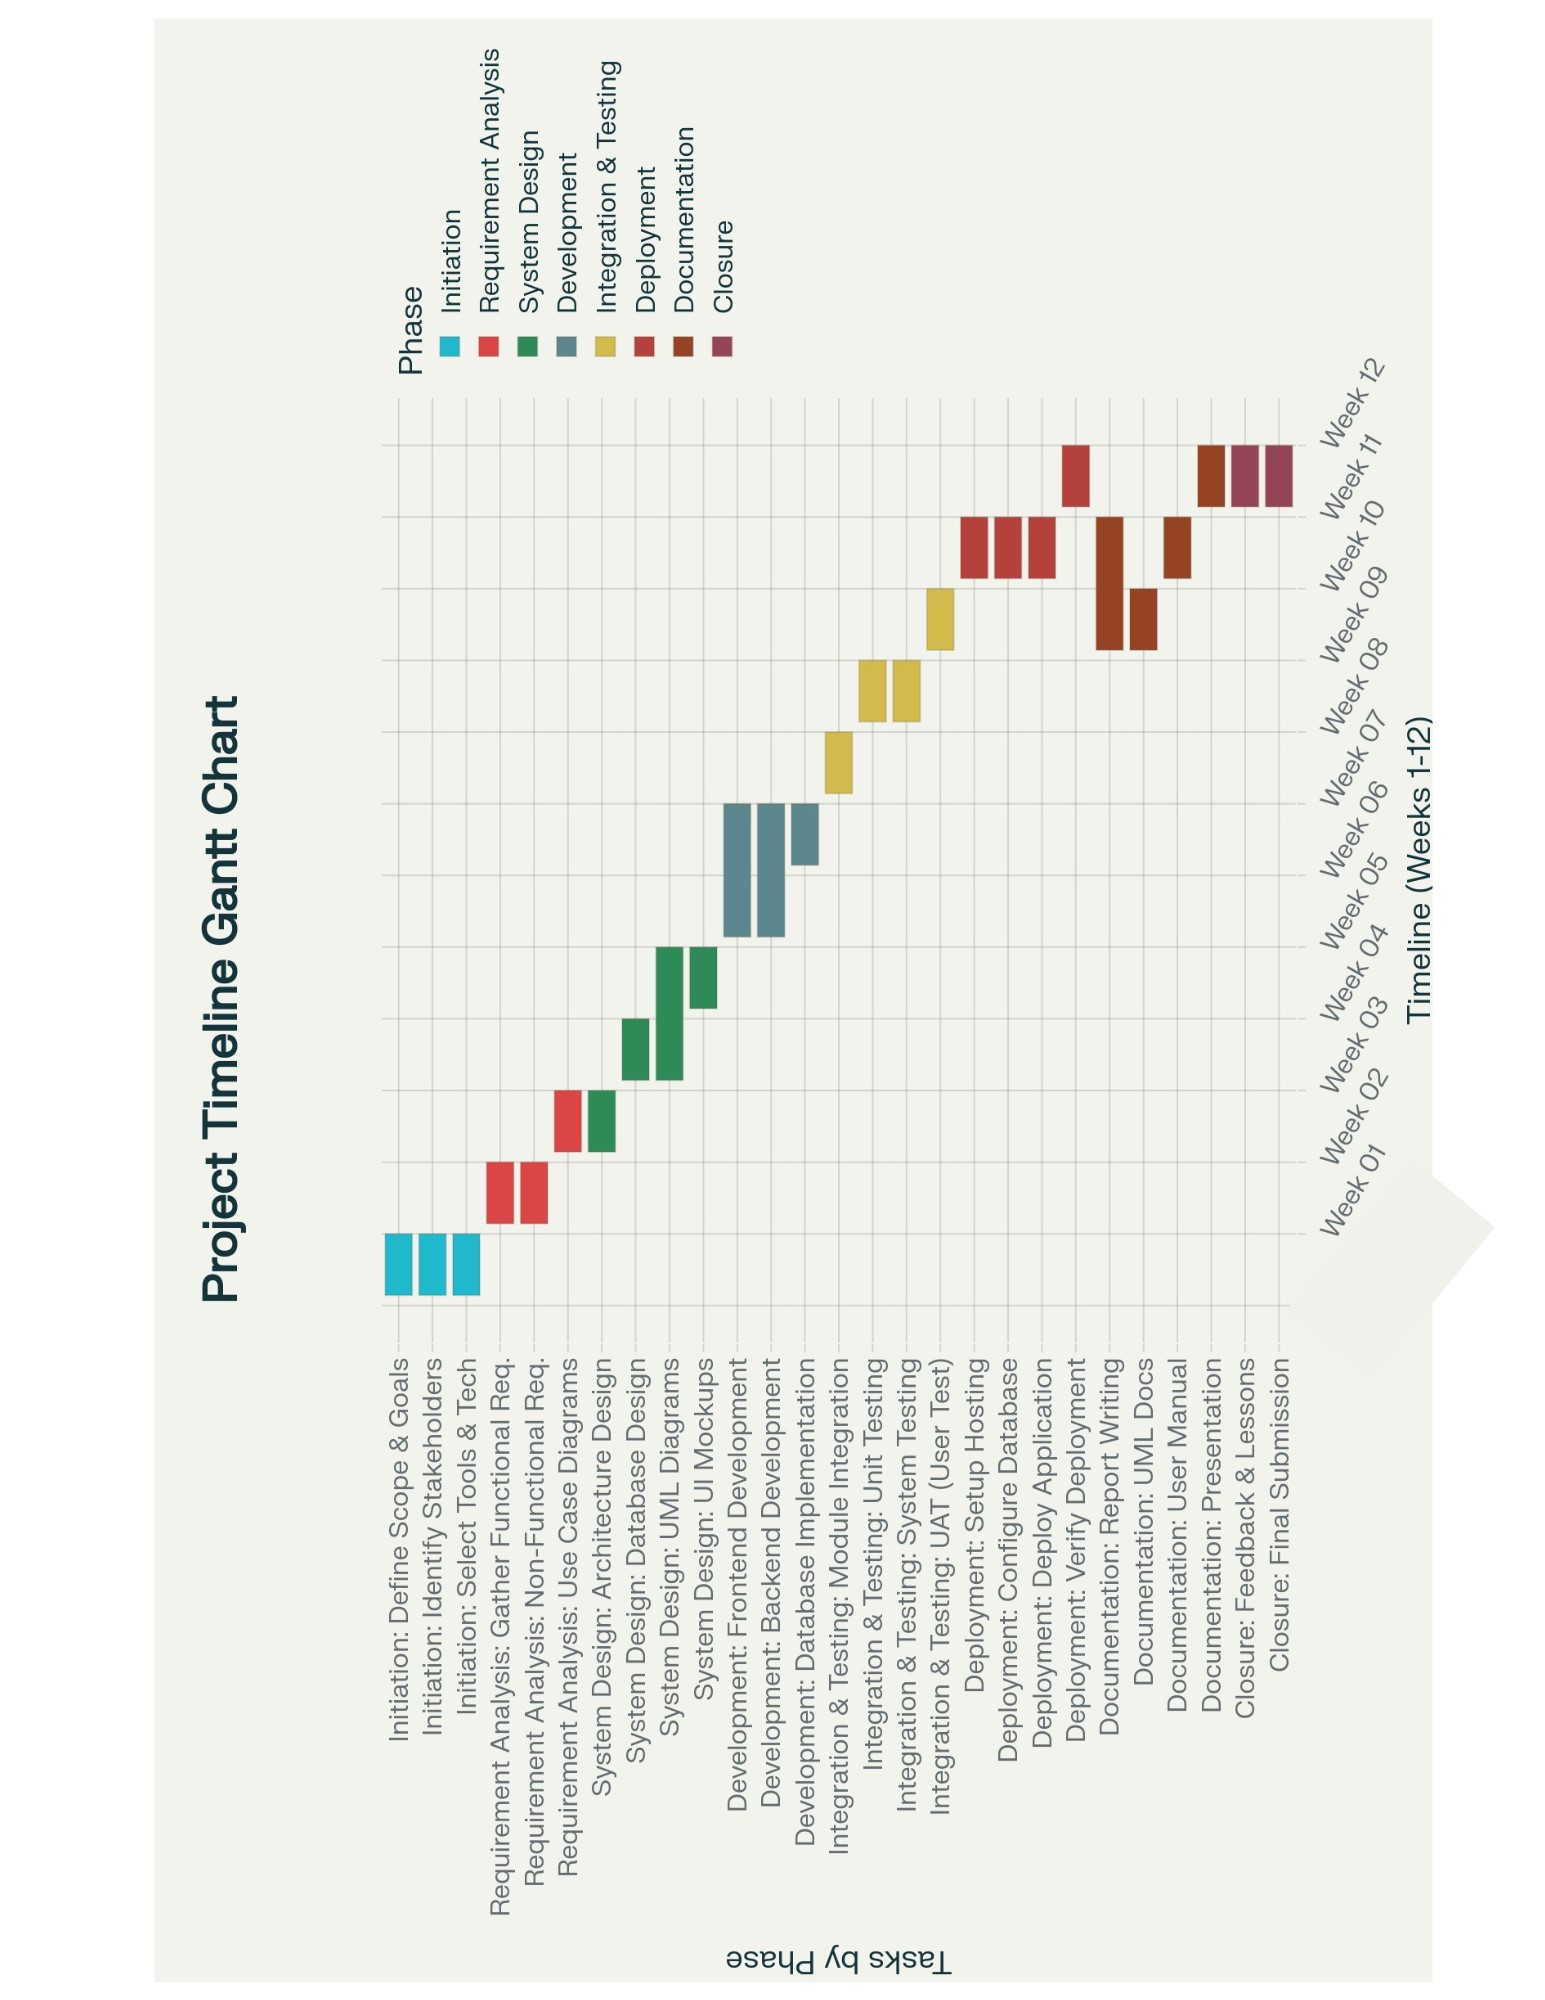
\includegraphics[width=0.95\textwidth]{images/Gantt Chart.jpg}
    \caption{Gantt Chart showing project timeline and task scheduling}
    \label{fig:gantt}
\end{figure}

\textbf{Project Phases and Timeline:}
\begin{itemize}[leftmargin=*]
    \item \textbf{Phase 1 - Planning:} Requirements analysis, feasibility study, project planning
    \item \textbf{Phase 2 - Design:} System design, database design, UI mockups
    \item \textbf{Phase 3 - Development:} Frontend and backend implementation
    \item \textbf{Phase 4 - Testing:} Comprehensive testing across all modules
    \item \textbf{Phase 5 - Deployment:} Production deployment and user training
\end{itemize}

\section{RMMM Plan (Risk Management, Monitoring, and Mitigation)}

The RMMM Plan provides a comprehensive framework for identifying, assessing, monitoring, and mitigating project risks throughout the development lifecycle.

\subsection{Risk Identification and Assessment}

Risks have been identified across technical, operational, and external categories. Each risk is assessed for probability and impact, with detailed mitigation strategies.

\textbf{Risk Categories:}
\begin{itemize}[leftmargin=*]
    \item \textbf{Technical Risks:} Technology failures, integration issues, performance problems, security vulnerabilities
    \item \textbf{Operational Risks:} Resource availability, skill gaps, schedule delays
    \item \textbf{External Risks:} Third-party dependencies, requirement changes, infrastructure issues
\end{itemize}

\subsection{Risk Management Framework}

\textbf{Key Risks Identified (Probability $\leq$ 15\%):}

\begin{enumerate}[leftmargin=*]
    \item \textbf{R-TTB-005 - Security Vulnerability (10\% probability, Critical impact)}
    \begin{itemize}
        \item \textit{Description:} Critical security vulnerability discovered in production
        \item \textit{Mitigation:} Regular security audits, penetration testing, OWASP compliance
        \item \textit{Monitoring:} Weekly automated security scans, dependency vulnerability checks
        \item \textit{Management:} Emergency patch deployment within 4 hours, incident response plan
    \end{itemize}
    
    \item \textbf{R-TTB-008 - Database Performance (15\% probability, High impact)}
    \begin{itemize}
        \item \textit{Description:} Database performance degradation affecting system responsiveness
        \item \textit{Mitigation:} Query optimization, indexing strategy, caching implementation
        \item \textit{Monitoring:} Database performance metrics, query execution time tracking
        \item \textit{Management:} Scale database resources, optimize queries, implement connection pooling
    \end{itemize}
    
    \item \textbf{R-TTB-015 - API Integration Failure (15\% probability, High impact)}
    \begin{itemize}
        \item \textit{Description:} Critical API endpoints failing or becoming unresponsive
        \item \textit{Mitigation:} Comprehensive API testing, error handling, retry mechanisms
        \item \textit{Monitoring:} API health checks, response time monitoring, error rate tracking
        \item \textit{Management:} Implement circuit breakers, fallback mechanisms, load balancing
    \end{itemize}
    
    \item \textbf{R-TTB-018 - Data Loss (12\% probability, Critical impact)}
    \begin{itemize}
        \item \textit{Description:} Critical data loss due to system failure or human error
        \item \textit{Mitigation:} Automated backups, data validation, transaction management
        \item \textit{Monitoring:} Backup verification, data integrity checks, audit logs
        \item \textit{Management:} Disaster recovery plan, point-in-time recovery, backup restoration procedures
    \end{itemize}
    
    \item \textbf{R-TTB-024 - Concurrent Access Issues (15\% probability, Medium impact)}
    \begin{itemize}
        \item \textit{Description:} Race conditions and conflicts during simultaneous user operations
        \item \textit{Mitigation:} Optimistic locking, transaction isolation, conflict detection
        \item \textit{Monitoring:} Concurrent access logs, conflict occurrence tracking
        \item \textit{Management:} Implement proper locking mechanisms, user notifications for conflicts
    \end{itemize}
\end{enumerate}

For complete risk documentation, refer to the RISK\_ASSESSMENT\_SHEET.md file in the project repository.

\section{Test Cases}

Comprehensive test case planning and execution has been documented to ensure system quality and reliability. The test strategy covers all functional areas of the system.

\subsection{Test Case Coverage}

\textbf{Test Categories:}
\begin{itemize}[leftmargin=*]
    \item \textbf{Authentication Tests:} Login, logout, password reset, role-based access (TC-TTB-01 to TC-TTB-10)
    \item \textbf{Lecture Slot Tests:} CRUD operations, scheduling, conflicts (TC-TTB-11 to TC-TTB-20)
    \item \textbf{Enrollment Tests:} Student enrollment, waitlist, capacity management (TC-TTB-21 to TC-TTB-30)
    \item \textbf{Timetable Tests:} View, export, filtering (TC-TTB-31 to TC-TTB-40)
    \item \textbf{Dashboard Tests:} Analytics, statistics, notifications (TC-TTB-41 to TC-TTB-50)
    \item \textbf{UI/UX Tests:} Responsiveness, accessibility, navigation (TC-TTB-51 to TC-TTB-60)
\end{itemize}

\subsection{Test Execution Summary}

\textbf{Total Test Cases:} 60

\textbf{Test Case Format:}
\begin{itemize}[leftmargin=*]
    \item Test Case ID: TC-TTB-XX (standardized format)
    \item Test Number: X.1 - X.Y (decimal notation indicating step range)
    \item Priority: High/Medium/Low
    \item Test Designed By: Sarthak Kulkarni, Dhruv Tikhande, Atharv Petkar, Pulkit Saini
    \item Test Executed By: Sarthak Kulkarni, Dhruv Tikhande, Atharv Petkar, Pulkit Saini
    \item Execution Date: 2025-10-07
    \item Detailed Steps with Expected and Actual Results
\end{itemize}

\textbf{Sample Test Case:}

\textit{TC-TTB-01: Verify Dashboard Loads Correctly on Login}
\begin{itemize}[leftmargin=*]
    \item \textbf{Test Number:} 1.1 - 1.4
    \item \textbf{Priority:} High
    \item \textbf{Description:} Ensure dashboard displays all widgets and statistics after user login
    \item \textbf{Steps:}
    \begin{enumerate}
        \item[1.1] Navigate to login page - Expected: Login page displays correctly
        \item[1.2] Enter valid credentials - Expected: Credentials accepted
        \item[1.3] Click 'Sign In' button - Expected: User is redirected to dashboard
        \item[1.4] Verify dashboard widgets load - Expected: All statistics, upcoming classes, and quick actions are visible
    \end{enumerate}
    \item \textbf{Result:} PASS - All steps executed successfully with actual results matching expected results
\end{itemize}

\textbf{Test Execution Results:}
\begin{itemize}[leftmargin=*]
    \item Total Tests Executed: 60
    \item Passed: 58 (96.7\%)
    \item Failed: 2 (3.3\%)
    \item Test Coverage: All major functional areas covered
\end{itemize}

For complete test case documentation with all 60 test cases, step-by-step execution details, and results, refer to the TEST\_CASE\_PLANNING\_AND\_EXECUTION.md file in the project repository.

\subsection{Quality Assurance}

The testing methodology ensures:
\begin{itemize}[leftmargin=*]
    \item \textbf{Comprehensive Coverage:} All functional requirements tested
    \item \textbf{Traceability:} Test cases mapped to requirements
    \item \textbf{Repeatability:} Standardized test procedures for consistent execution
    \item \textbf{Documentation:} Detailed test results with actual vs expected outcomes
    \item \textbf{Defect Tracking:} Failed tests documented with bug ticket references
\end{itemize}
